\documentclass[titlepage]{article}

\usepackage[utf8]{inputenc}
\usepackage{scrextend}
\usepackage[bottom]{footmisc}
\usepackage{graphicx}
\usepackage{float}
\usepackage{listings}

\title{Comfy: Gestionnaire de fenêtres par pavage}
\author{Daniel-Junior Dubé et Félix Chabot}
\date{Session d'automne 2018}

\graphicspath{ {./images/} }

\lstset{frame=single,numbers=left,inputpath=./sources}

\begin{document}
\maketitle

\renewcommand{\contentsname}{Table des matières}
\tableofcontents
\newpage

\section{Introduction}
\par
\bigskip
En tant qu'enthousiastes des systèmes d'exploitation GNU/Linux depuis quel-ques années, nous avons pu observer l’engouement de la communauté envers les gestionnaires de fenêtre en tuiles\footnote{https://en.wikipedia.org/w/index.php?title=Tiling\_window\_manager}. En effet, ces gestionnaires permettent une plus grande flexibilité pour la personnalisation de l’expérience utilisateur que les environnements de bureau populaire tel que \textit{Gnome}, \textit{KDE} et \textit{Xfce} tout en étant plus léger sur l’utilisation des ressources matérielles. Tout comme les outils minimalistes tel \textit{Vim} et \textit{Emacs}, ces gestionnaires de fenêtres permettent aussi de bénéficier à l’efficacité des développeurs qui les utilisent grâce aux nombreux raccourcis clavier.

\par
\bigskip
De plus, le tout nouveau protocole de serveur d'affichage \textit{Wayland} est de plus en plus adopté par ces environnements de bureau. Celui-ci est perçu par plusieurs comme un candidat idéal pour remplacer le protocole \textit{X} d'ici quelques années à cause de son architecture optimisée et pour sa meilleure gestion des ressources matérielles.

\par
\bigskip
Dans le cadre de ce projet, nous avons donc décidé de concevoir un gestionnaire de fenêtres utilisant ce nouveau protocole et celui-ci sera écrit avec le langage de programmation \textit{Rust}. Ce langage apporte des fonctionnalités modernes intéressantes en ce qui concerne la gestion mémoire, la concurrence et la gestion de dépendance, tout en gardant une performance rivalisant celle du \textit{C} et \textit{C++}. Il existe peu de gestionnaires de fenêtres utilisant à la fois \textit{Rust} et \textit{Wayland}. Il y en a un en particulier s’appelant \textit{Way-Cooler}\footnote{http://way-cooler.org}, mais selon les auteurs de ce projet, il n’est pas encore assez stable pour être utilisé en “production”.

\par
\bigskip
Notre but sera donc de créer un logiciel que des enthousiastes pourront ultimement utiliser dans leur quotidien tout en nous permettant d’apprendre les rudiments de la programmation de composante système.

\section{Revue de littérature}
\begin{description}
	\item [Gestionnaire de fenêtre] Un logiciel qui contrôle l’affichage et la disposition des fenêtres des applications en exécution.
	\item [Écran] Un écran est un espace de rendu qui est mis à notre disposition via un appareil physique (moniteur).
	\item [Espace de travail] Un écran possède une liste d’espaces de travail. Un seul espace de travail est affiché à l’écran à la fois et l'utilisateur peut déterminer lequel sera affiché.
	\item [Fenêtre] Une fenêtre est une feuille dans l’arbre de disposition. Elle est donc l’espace réservé à l’affichage du rendu d’une application en exécution.
	\item [Gestionnaire de disposition de fenêtres]
			Un espace de travail est constitué d’une seule disposition de fenêtre. Celle-ci applique des contraintes d'affi-chage sur les fenêtres qu'elle contient en ce qui concerne avec la position et la dimension de celles-ci.
	\item [Arbre de disposition de fenêtres] Implémentation du gestionnaire de disposition de fenêtres utilisant un arbre enraciné (k-ary tree).
	\item [Noeud de disposition (dans l’arbre de disposition)] Noeud dans l’arbre de la disposition. Correspond essentiellement à un conteneur de fenêtres et sous-noeuds.
	\item [Tuile] Correspond à l’espace (ou subdivision) de l’écran réservé à une  fenêtre.
	\item [Subdivision] Une subdivision représente à la fois un noeud dans l’arbre de disposition et un sous-ensemble de l’espace d’affichage de l’écran.
	\item [Conteneur de fenêtres] Un conteneur est un noeud dans l’arbre de disposition. Il s’agit donc d’une structure de données qui va contenir un ensemble de fenêtres ou de sous-conteneurs.
	\item [Liaison de touche (Keybinding)] Représente l'association d'une combinaison de touches à une commande de l'application.
	\item [Commande] Fonctionnalité du gestionnaire de fenêtre accessible à l'utilisateur via une combinaison de touche.
	\item [Pointeur] Un appareil physique servant à envoyer des évènements de mouvement au compositeur. Très souvent il s'agit d'une souris, mais pourrait être un écran tactile.
	\item [Curseur] Une image représantant l'emplacement du pointeur dans le compositeur.
	\item [Indicateur d'insertion] Une représentation visuelle de la direction d'insertion relative à la fenêtre active.
	\item [Fenêtre active] Fenêtre possédant le focus, c'est-à-dire qui reçoit les évène-ments des appareils d'entrées (clavier, souris, etc ...).
\end{description}

\section{Installation}
Afin d'installer \textit{Comfy}, la première étape est de s'assurer que l'utilisateur poss-ède toutes les dépendances de \textit{wlroots}\footnote{https://github.com/swaywm/wlroots}. Ensuite, il faut tout simplement utiliser le fichier \textit{Makefile} de la façon suivante :
\begin{verbatim}
	$ make
	$ sudo make install
\end{verbatim}

\par
Celui-ci s'occupera de compiler et copier les différents fichiers aux bons emplacements systèmes. Les indications d'installation les plus récentes sont situées dans le fichier \textit{README.md}.

\section{Manuel d'utilisateur}
Comme toute application \textit{UNIX} qui se respecte, \textit{Comfy} possède un manuel d'utilisateur accessible à l'aide la commande \textit{man}.

\begin{verbatim}
	$ man confywm
\end{verbatim}

\section{Diagrammes du fonctionnement}
\begin{figure}[H]
	\centering
	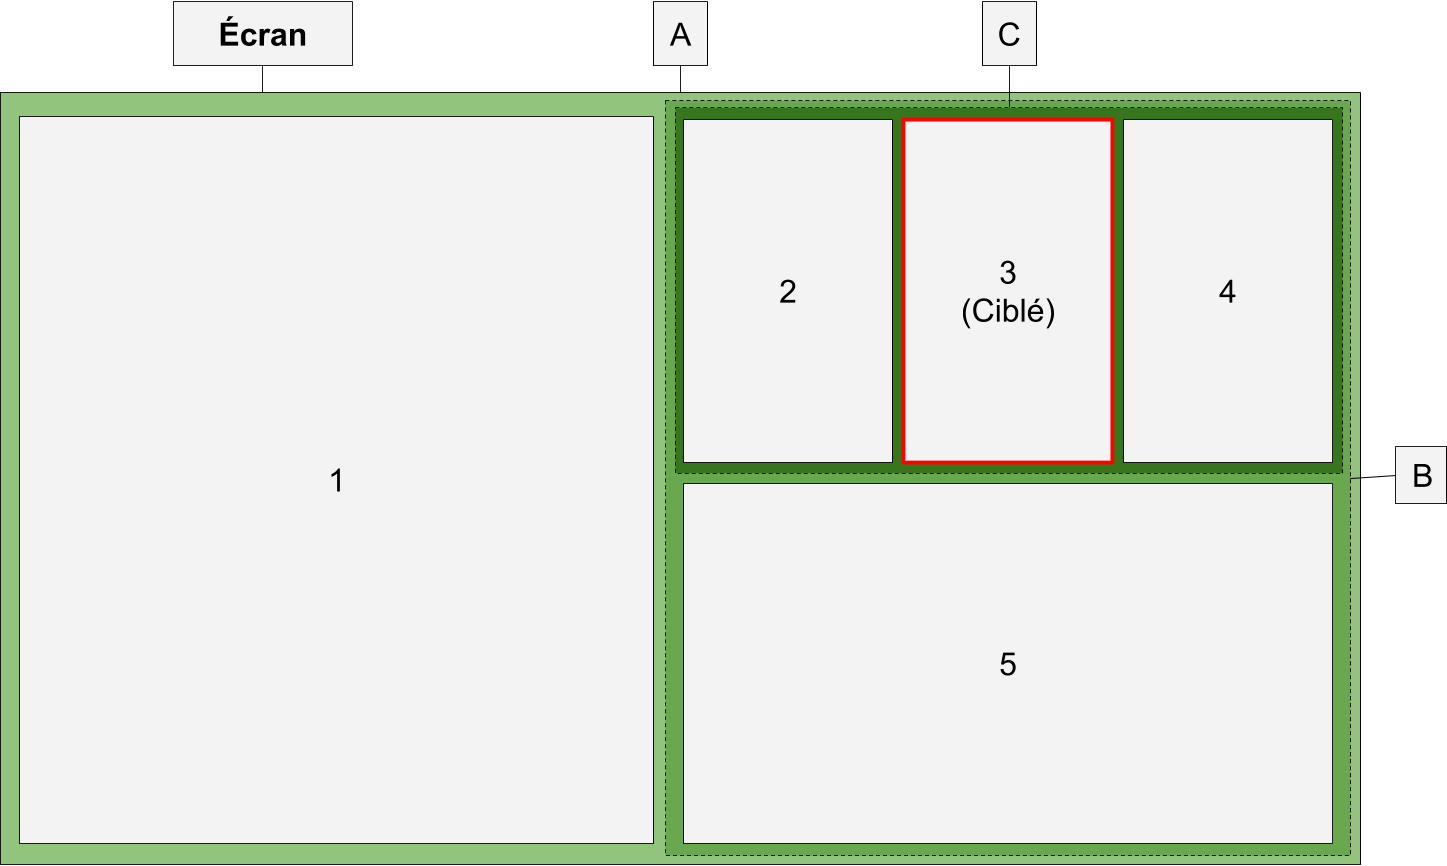
\includegraphics[width=\textwidth]{diagramme_du_fonctionnement.png}
	\caption{Représentation de l'état de la disposition de fenêtre}
\end{figure}
\begin{figure}[H]
	\centering
	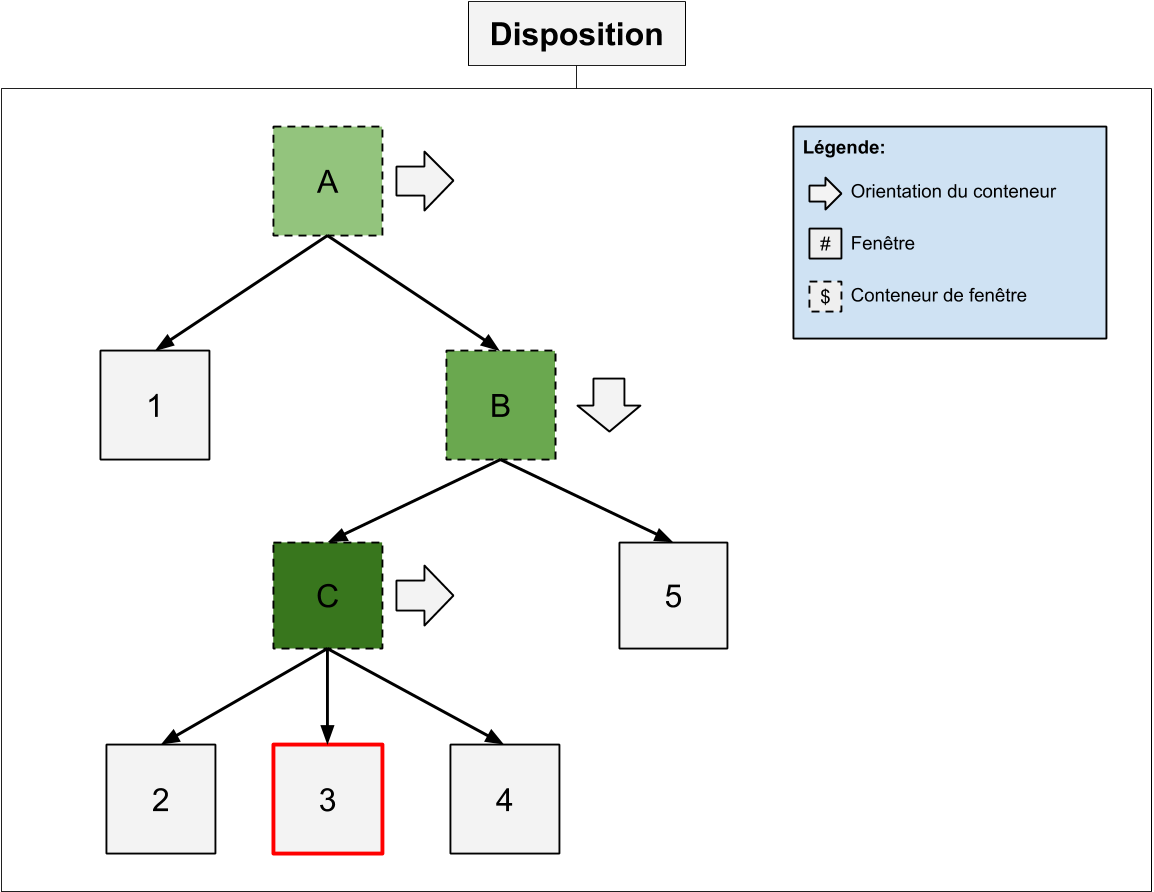
\includegraphics[width=\textwidth]{diagramme_du_fonctionnement_arbre.png}
	\caption{Arbre résultant}
\end{figure}

\section{Composantes}
\subsection{Configuration}
\par
\bigskip
Afin de donner une meilleure expérience aux utiliseurs de \textit{Comfy}, nous avons décidé de laisser la possibilité de pouvoir personaliser un grand nombre de fonctionnalités à même l'application. Le format des fichiers de configuration utilisera \textit{TOML}\footnote{https://github.com/toml-lang/toml}. Ce format est d'ailleurs utilisé pour les fichiers de configuration du langage \textit{Rust}. \textit{TOML} est très similaire au \textit{YAML} et \textit{JSON} pour la représentation des différents types de données et de la simplicité d'écriture. Par contre, \textit{TOML} porte une plus grande importance à la lisibilité ce qui est un point cruciale pour un fichier de configuration. De plus, il est possible de rajouter des commentaires aux fichiers d'exemple ce qui va nous permettre de bien expliquer les configurations possibles aux utilisateurs. Pour l'instant nous avons les fichiers de configurations suivants:
\begin{itemize}
	\item Un fichier pour les options globales de l'application \textbf{global.toml}
	\item Un fichier pour les raccourcis clavier appelé \textbf{keybings.toml}
	\item Un fichier pour l'apparence de \textit{Comfy} appelé \textbf{theme.toml}
\end{itemize}

\subsubsection{global.toml}
\begin{minipage}{\linewidth}
	\lstinputlisting[label=global-example,title=Exemple d'un fichier
	global.toml]{global.toml}
\end{minipage}

\par
Ce fichier représente les attributs personnalisables associés au comportement général de l'application. Voici la définition des attributs pouvant être personnalisés:
\begin{description}
	\item [pointer\_focus\_type] Détermine de quelle façon l'intéraction du pointeur influence le focus des fenêtres.
\end{description}

\subsubsection{keybindings.toml}
\begin{minipage}{\linewidth}
	\lstinputlisting[label=keybindings-example,title=Exemple d'un fichier
	keybindings.toml]{keybindings.toml}
\end{minipage}

\par
Un paramètre important de ce fichier de configuration est \textit{modkey} qui va servir à définir une sorte de macro utilisable tout au long du fichier. Pour faire référence au \textit{modkey} il faut seulement entrer \textit{\$mod} à l'intérieur d'une chaîne de combinaison de touche et \textit{Comfy} s'occupera de remplacer cette référence à la touche associée précédement. L'utilité du \textit{modkey} est de dédier de façon simple une touche centrale de contrôle pour les commandes de \textit{Comfy}. Une touche parfaite pour le \textit{modkey} serait une touche modificatrice\footnote{https://fr.wikipedia.org/wiki/Touche\_de\_combinaison} comme les touches \textbf{Control}, \textbf{Super} et \textbf{Alt} car celles-ci ne devraient pas avoir un impact sur le fonctionnement des applications sous-jacentes.
\par
\bigskip
Ensuite, nous avons la section \textbf{keybindings}. Cette section sera la partie la plus importante du fichier, car c'est elle qui comprend la définition des associations des combinaisons de touches aux commandes. Une entrée de cette section est relativement simple. Le membre gauche de l'association est un ensemble de touches sous la forme d'une chaîne de caractère (entre guillemets) utilisant le caractère séparateur '+'. Malheureusement, la clé en \textit{TOML} (qui est le membre gauche en question) ne peut pas contenir ce symbole, c'est pourquoi nous utilisons la représentation en chaîne de caractère. Ensuite, le membre droit contient deux parties, une commande suivie de ses arguments. Par exemple, à la ligne 4 du fichier d'exemple, nous avons:

\lstinputlisting[frame=none,numbers=none,firstline=4,lastline=4]{keybindings.toml}

La commande serait donc \textbf{exec} et l'argument serait \textbf{weston-terminal}.

\par
\bigskip
Une chose importante à savoir est que \textit{Comfy} gère les entrées clavier et vérifie si une combinaison de touches se trouve dans le fichier de configuration et l'exécute. Ceci serait problématique si le même raccourci serait aussi associé dans une application. Par exemple, associer une commande à la combinaison \textbf{Control+s} (un raccourci populaire pour enregistrer un fichier) ne serait pas une bonne idée puisque celle-ci sera toujours interceptée par \textit{Comfy} avant même de se rendre à l'application.

\subsubsection{theme.toml}
\begin{minipage}{\linewidth}
	\lstinputlisting[label=theme-example,title=Exemple d'un fichier theme.toml]{theme.toml}
\end{minipage}

\par
Ce fichier représente les attributs visuels personnalisables de l'application. Voici la définition des attributs pouvant être personnalisés:
\begin{description}
	\item [border\_size] Détermine l'épaisseur des bordures autour d'une fenêtre à l'in-térieur d'une tuile.
	\item [active\_color] Couleur de la bordure autour de la fenêtre active.
	\item [inactive\_color] Couleur de la bordure autour des fenêtres non-actives.
	\item [cursor\_indicator\_color] Couleur du côté de la bordure de la fenêtre active indiquant l'emplacement d'insertion des fenêtres.
	\item [wallpaper\_path] Chemin vers le fichier de l'image qui sera utilisée comme fond d'écran.
\end{description}

\section{Tests}
Étant donné la nature du projet, une application graphique de bas niveau, plusieurs composantes sont difficilement testable à l'aide de tests d'intégration. En effet, nous avons d'avantage utilisé des tests fonctionnelles pour s'assurer du bon fonctionnement d'un module. Il existe toutefois une exception avec le module de configuration. Dans ce module, nous avons intégré des tests unitaires pour nous assurer que nos fonctions génèrent les bonnes configurations. Un avantage d'utiliser \textit{Rust} est que les tests unitaires sont supportés nativement. Pour exécuter la suite de test, il suffit d'entrer cette commande :
\begin{verbatim}
	$ cargo test
\end{verbatim}

\section{Organisation du code source}
Le projet étant d'une taille considérable, nous avons essayé de le subdiviser le plus possible en sous-section. Voici les majeurs répertoires :
\begin{description}
	\item [config] Répertoire contenant les fichiers de configuration par défaut. Ces fichiers vont être copiés lors de l'installation afin de devenir les configuration du système.
	\item [data] Répertoire contenant d'autres fichiers nécessaires pour l'installation sys-tème. Par exemple, il y a un \textit{Desktop Entry} servant à lancer l'application à partir d'un \textit{X Display Manager}.
	\item [doc] Répertoire contenant ce rapport.
	\item [lib] Répertoire contenant la librairie \textit{wlroots-rs} sous-forme d'un sous-module \textit{git}.
	\item [src] Répertoire contenant le code source de \textit{Comfy}. Nous allons entrer plus en détails sur ce répertoire dans la section suivante.
	\item [target] Répertoire contenant le code compilé de \textit{Comfy}.
\end{description}

Mis-à-part ces dossiers, il y a quelques fichiers importants se trouvant dans la racine du projet :
\begin{description}
	\item [Cargo.toml] Le fichier de configuration du projet \textit{Rust}, il contient notamment les dépendances du code source.
	\item [Makefile] Le fichier servant à compiler et installer l'application sur le système.
\end{description}
\subsection{Description du répertoire ``src"}
\begin{description}
	\item [comfy] Le répertoire principale du code source. Tous ses sous-répertoires re-présentent des modules de \textit{Comfy}. Par exemple, le sous-répertoire \textit{input} contient les implémentations du clavier et de la souris. Se mode de fonctionnement est largement dicté par \textit{Rust}.
	\item [common] Un repertoire contenant des éléments partagés pouvant être utilisé pour des projets externes (des scripts utilisateurs par exemple).
	\item [lib.rs] Un fichier \textit{Rust} servant à partager les fichiers contenus dans \textit{common}.
\end{description}

\section{Analyse/Conception}
\par
Comme la phase de recherche et d'analyse a occupé le tier du temps alloué au développement du projet, nous avons réalisé une quantité considérable de schémas et de documents de recherche. Ceux-ci nous ont permis de partager efficacement notre vision des éléments de conception.
\bigskip

\par
En premier lieu, nous avons notre prototype de diagramme de classes initial:
\bigskip

\begin{figure}[H]
	\centering
	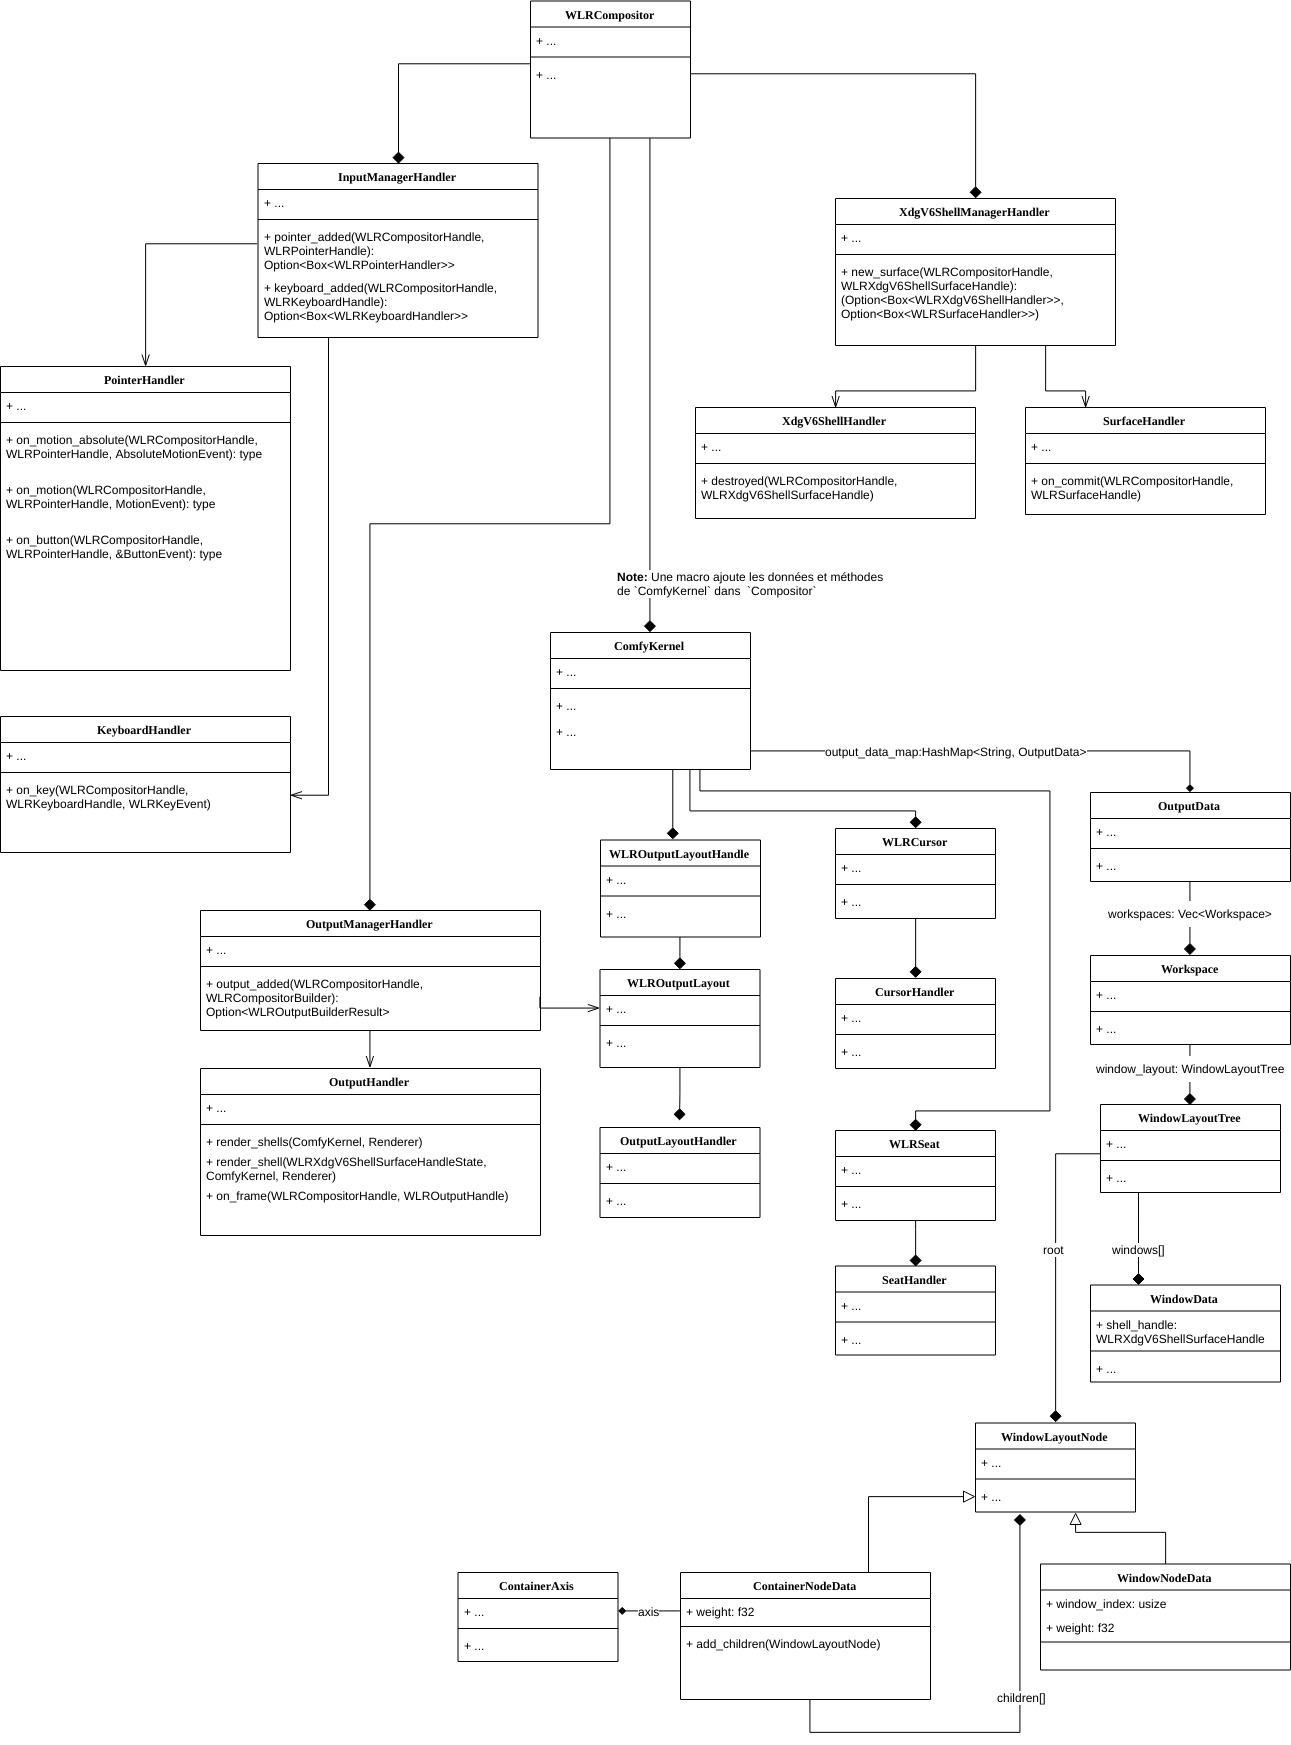
\includegraphics[width=\textwidth]{Diagramme_de_classes.jpg}
	\caption{Prototype du diagramme de classes}
\end{figure}

\par
Grâce à ce diagramme, nous pouvons observer la répartition des responsabilités à travers les différentes composantes du système. Par exemple, nous observons à gauche les classes qui gèrent les évènements des entrées, qui sont associés à la racine du compositeur.
\bigskip

\par
Les autres schémas concernant la conception de l'application se retrouvent dans la section suivante "Architecture", car même si ceux-ci ont fait parti de la phase d'analyse et conception, ils ont évolués tout au long du projet pour correspondre ultimement à l'état actuel de notre architecture.
\bigskip

\section{Architecture}
\subsection{Architecture générale}
\par
Afin de comprendre le fonctionnement de notre application au plus haut niveau possible, voici le schéma d'architecture générale:
\bigskip

\begin{figure}[H]
	\centering
	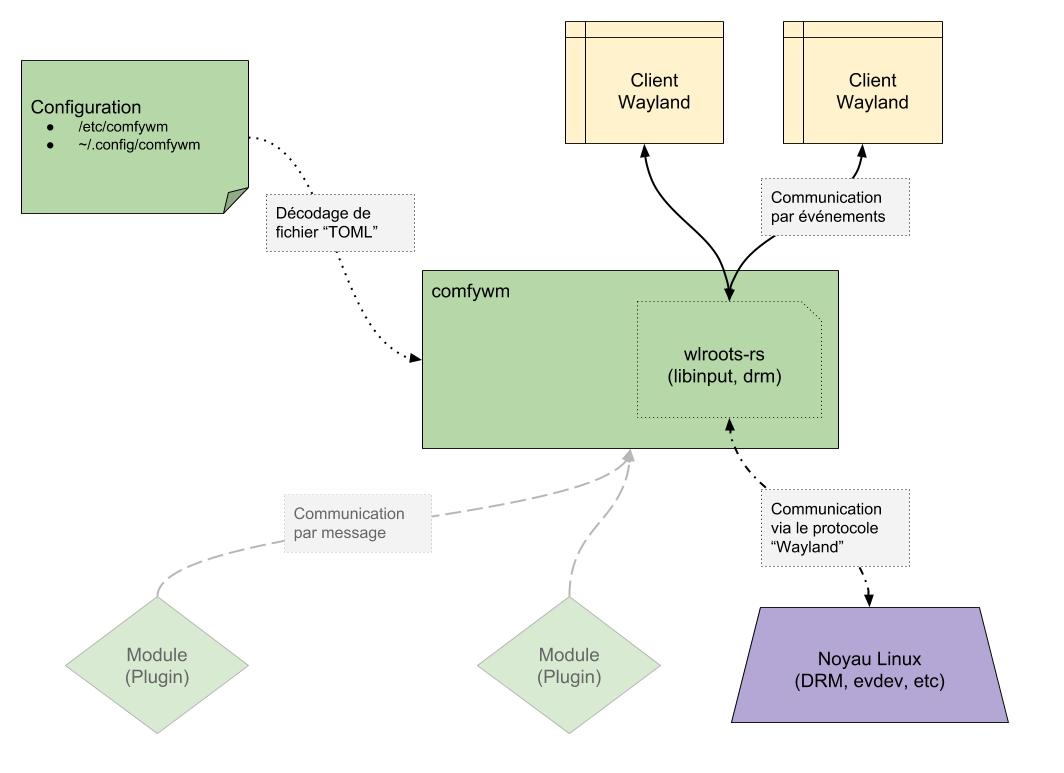
\includegraphics[width=\textwidth]{architecture_generale_v1.jpg}
	\caption{Architecture générale}
\end{figure}

\par
Dans cette image, nous observons qu'il y a quatres formes en vert. Celles-ci représentent les composantes faisant partie de l'implémentation de Comfy. Par contre, les éléments grisâtres représentant les éléments qui ont été abandonnés au fil du projet.
\bigskip

\subsubsection{Composante de base}
\par
Le prochain schéma représente la fondation de l'implémentation de notre compositeur avec la sous-struture de base, le \textbf{ComfyKernel}.
\bigskip

\begin{figure}[H]
	\centering
	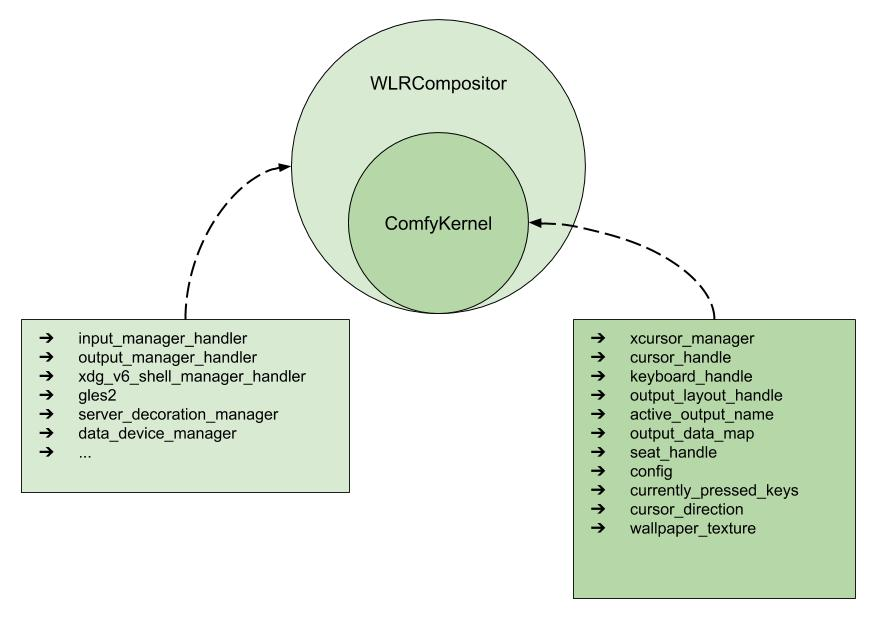
\includegraphics[width=\textwidth]{architecture_base.jpg}
	\caption{Composante de base}
\end{figure}

\par
Pour l'instant, le \textit{ComfyKernel} possède beaucoup trop de responsabilités, dont la réécriture sera l'un des premiers objectifs de la continuation du projet. Par contre, comme la structure du compositeur est accessible à partir de chaque gestionnaire d'évènement, l'implémentation actuelle nous permet d'accéder facilement aux différentes données partagées.
\bigskip

\subsubsection{Intération utilisateur}
\par
Le concept illustré ci-dessous représente un part assez complexe du comportement de notre compositeur, la gestion de l'intération de l'utilisateur avec l'appli-cation.
\bigskip

\begin{figure}[H]
	\centering
	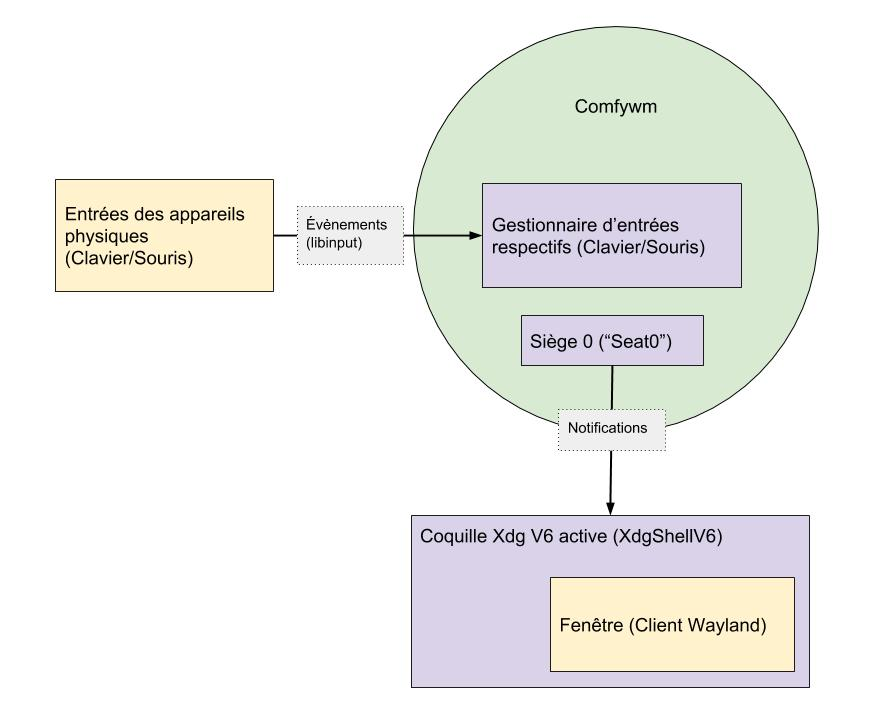
\includegraphics[width=\textwidth]{interaction_utilisateur.jpg}
	\caption{Intération utilisateur}
\end{figure}

\par
Grâce à l'implémentation de \textit{wlroots}, nous avons directement accès aux méthodes de support des évènements émis par \textit{libinput}, la bibliothèque système qui gère les données reçues par les appareils d'entrées (clavier, souris, pavé tactile, etc).
\bigskip

\subsubsection{Sorties et espaces de travail virtuels}
\par
Lors de la réception d'un évènement de création d'un appareil d'affichage (dans notre cas, l'écran ou la sortie), nous ajoutons une entrée dans la structure associant le nom de l'écran et ses données. Cette entrée possède les données de l'espace de travail actuel de l'écran qui pour sa part, contient le gestionnaire de disposition des fenêtres.
\bigskip

\begin{figure}[H]
	\centering
	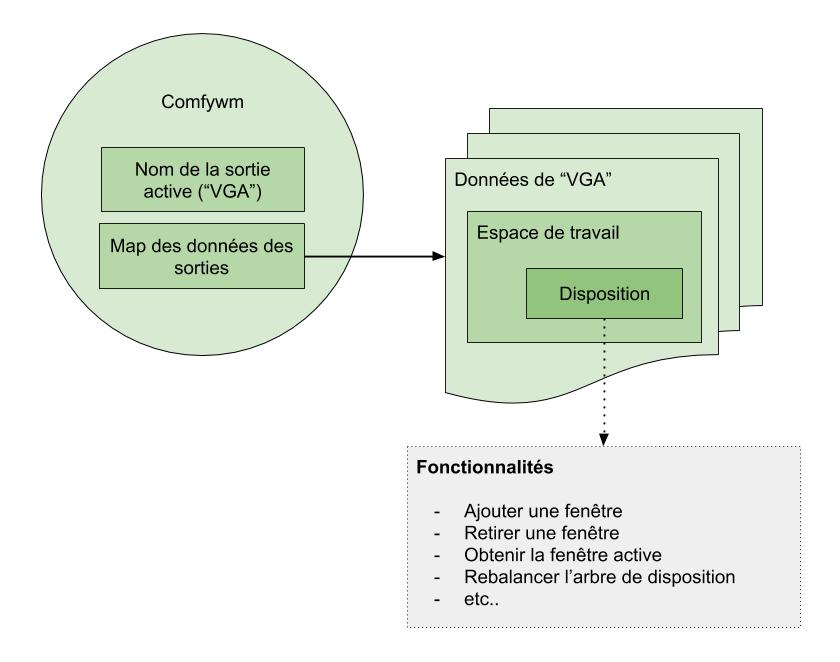
\includegraphics[width=\textwidth]{sorties_et_espaces_de_travail.jpg}
	\caption{Sorties et espaces de travail}
\end{figure}

\subsubsection{Disposition des fenêtres}
\par
Lorsqu'une application sous-jacentes est exécutée et qu'une surface d'affichage est fournie, la coquille associée à celle-ci est envoyé dans le gestionnaire de disposition actif (celui contenu dans l'écran avec lequel nous intéragissons). Le gestionnaire en question se chargera d'appliquer les contraintes d'affichage. Ensuite, lorsqu'un évènement de rendu sera perçu pour l'écran en question, le gestionnaire de disposition sera prêt à fournir les "poignées" vers les fenêtres à afficher.
\bigskip

\par
Notre implémentation se base sur une structure nommée "Arbre enraciné" qui, afin de respecter efficacement les restrictions de partage de référence de \textit{Rust}, est basé sur un entreposage de noeud par région (appelé "region-based" ou "arena-based"). L'aire de chaque noeud est calculé via l'aire du parent et du ratio de son poid par rapport à ses voisins. L'orientation de chaque noeud est controllé par son conteneur, c'est-à-dire, le noeud parent. Seul les feuilles sont associées à des fenêtres d'application.
\bigskip

Voici un schéma illustrant le fonctionnement:

\begin{figure}[H]
	\centering
	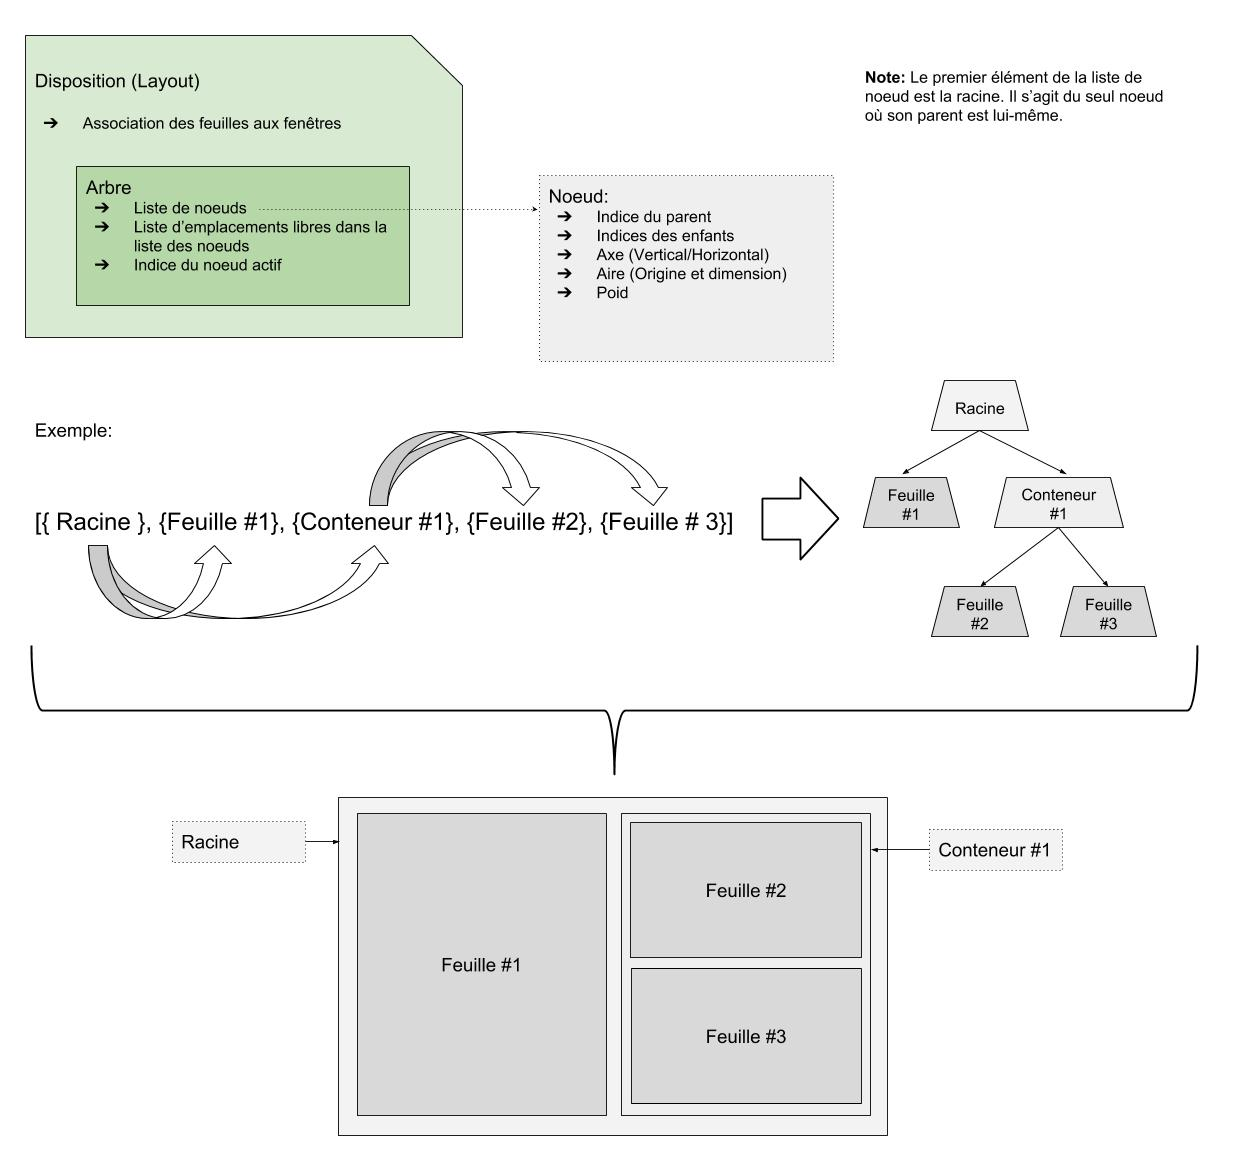
\includegraphics[width=\textwidth]{arbre_de_disposition.jpg}
	\caption{Disposition des fenêtres}
\end{figure}

\section{Conclusion}
\par
En ce qui concerne le résultat obtenu au bout de nos 15 semaines de travail, nous sommes très satisfait du produit final. Nous avons aussi reçu une excellente rétroaction de nos camarades de classe. Nous sommes convaincus que ce succès est majoritairement dû à la méthodologie que nous avons employée. Le fait de réserver près du tier du projet à la recherche, l'analyse et l'expérimentation nous a grandement aidé à évaluer correctement le poids des différentes tâches à accomplir. Les différentes phases de réécriture effectuées sur les implémentations expérimentales ont contribué à l'amélioration de la qualité du code et à renforcer la compréhension générale des membres de l'équipe.
\bigskip

\par
Il est aussi important de mentionner le rôle crucial de la communauté lors de la résolution de certains problèmes majeurs rencontrés. Leur contribution et leur support tout au long du projet furent essentiels à notre réussite. Nous espérons être en mesure de finaliser et de perfectionner l'application afin de pouvoir offrir un produit de qualité à la communauté. Pour cela, plusieurs autres itérations seront nécessaires, mais étant donné le progrès observé au cours des 15 dernières semaines, nous croyons qu'il s'agit d'un objectif tout à fait réalisable.
\bigskip

\section{Lien repris avec la formation}
Notre projet étant de plutôt grande envergure, nous avons utilisé beaucoup de concepts appris tout au long de notre formation. Notamment ceux appris lors du cours de système d'exploitation étant donné que nous avons développé une application système. Les notions d'évènements ont été particulièrment utile pour le module de gestion du clavier et de la souris. Ensuite, pour l'arbre de disposition le cours de structure de données fût essentiel puisque l'arbre utilise un ``Arbre enraciné". Bien entendu, ce n'est qu'une simple énumération des concepts clés que nous avons utilisés, la formation montre d'avantage comment résoudre des problèmatique de manière efficace.

\end{document}
